\documentclass[12pt,a4paper]{article}
\usepackage{amsmath}
\usepackage{amssymb}
\usepackage{amsthm}
\usepackage{graphicx}
\usepackage{tikz}
\usetikzlibrary{shapes.geometric, positioning, automata}
\usepackage{listings}
\usepackage{hyperref}
\usepackage{glossaries}
\usepackage[margin=1in]{geometry}
\usepackage{amssymb} % For checkmark symbol

% Define theorem environment
\newtheorem{theorem}{Theorem}

% Configure listings
\lstset{
    basicstyle=\ttfamily\small,
    breaklines=true,
    frame=single,
    numbers=left,
    numberstyle=\tiny\color{gray}
}

\makeglossaries

% Key Term Definitions
\newglossaryentry{flash}{
    name={Flash},
    description={A cognitive resonance event where brainwave patterns match a recognizable state threshold. Measured as a confidence percentage with target accuracy of 95.4\%}
}

\newglossaryentry{filter}{
    name={Filter},
    description={Processing mechanism that validates and categorizes brainwave data against known patterns before flash recognition}
}

\newglossaryentry{flashmodel}{
    name={Flash Model Engine},
    description={Core pattern matching system that processes EEG data to identify cognitive resonance states}
}

\newglossaryentry{objective_flash}{
    name={Objective Flash},
    description={Quantifiable brainwave pattern validated by AI Validator against measurable EEG metrics (delta, theta, alpha, beta, gamma waves)}
}

\newglossaryentry{subjective_flash}{
    name={Subjective Flash},
    description={User-interpreted meaning of flash event, maintaining interpretive authority with the dreamer}
}

\newglossaryentry{obicall}{
    name={OBICall},
    description={Polyglot AI binding layer that interfaces between core LLM and Dream System components. Executes as \texttt{obicall.exe [command] [subcommand]}}
}

\newglossaryentry{obiai}{
    name={OBIAI Agent},
    description={Intelligent actor operating within OBI framework, providing epistemic validation without imposing interpretation}
}

\newglossaryentry{ea_actor}{
    name={Epistemic Agent (EA) Actor},
    description={Non-AI clone that responds only to validated flash states with explicit user intent. Measures authenticity and coherence using flash confidence metrics}
}

\newglossaryentry{u_interface}{
    name={U (You)},
    description={Personalized AI dream interface enabling dialog between user and dream-self. Named to emphasize user agency and self-reflection}
}

\newglossaryentry{cognitive_observability}{
    name={Cognitive Observability},
    description={Non-invasive monitoring and interpretation framework for dream-state data using contextual brainwave metrics}
}

\newglossaryentry{non_invasive}{
    name={Non-invasive EEG},
    description={Surface electrode technology that captures brainwave activity without penetration of skin or tissue. Compliant with IEEE 11073 PHD standards}
}

\newglossaryentry{phone_orchestrator}{
    name={Phone Orchestrator},
    description={Mobile application serving as Bluetooth hub and network gateway, managing device connections and optimizing data transmission based on network quality (3G/4G/5G)}
}

\newglossaryentry{pedometric}{
    name={Pedometric Tracking},
    description={Continuous monitoring of physical activity metrics including steps, distance, heart rate, and activity classification for dream contextualization}
}

\newglossaryentry{family_investment}{
    name={Family Investment Channel},
    description={Authorized distribution pathway enabling dream sharing with trusted family members, supporting milestone-based engagement per OBINexus Legal Policy}
}

\newglossaryentry{true_remembrance}{
    name={True Remembrance Protocol},
    description={Multi-modal export system ensuring authentic dream recall through temporal anchoring, context preservation, and conversational memory}
}

\newglossaryentry{nsibidi}{
    name={Nsibidi},
    description={Ancient writing system of the Niger-Congo region, used in Dream System for symbolic verb-noun pairing to extract cultural meaning from dream events}
}

\newglossaryentry{csl}{
    name={Conceptual Symbolic Layer (CSL)},
    description={AI interpretation layer using Nsibidi verb-noun relationships to understand dream symbolism through Igbo cosmological framework}
}

\newglossaryentry{epistemic_cost}{
    name={Epistemic Cost Function},
    description={Mathematical function that measures the computational and interpretive cost of validating dream states. Used to determine when EA Actor should engage versus remain passive. Cost increases with ambiguity and decreases with confidence}
}

\newglossaryentry{flash_filter_dag}{
    name={Flash-Filter DAG},
    description={Directed Acyclic Graph structure organizing dream memory processing. Nodes represent flash events, edges represent temporal and causal relationships. Enables efficient retrieval and pattern matching across dream sequences}
}

\newglossaryentry{obicall_voip}{
    name={OBICall-VOIP},
    description={Voice over IP protocol extension for OBICall system. Enables real-time voice interaction between user and U agent upon waking. Implementations include pyobicall-voip (Python), node-obicallvoip (Node.js)}
}

\newglossaryentry{dimensional_game_theory}{
    name={Dimensional Game Theory},
    description={Multi-domain strategic reasoning framework enabling scalar-to-vector transitions in variadic action spaces. Allows EA actors to navigate complex decision landscapes with epistemic validation}
}

\newglossaryentry{cryptographic_primitive}{
    name={Cryptographic Primitive},
    description={Fundamental building block of cryptographic systems (hashing, KDF, encryption) standardized through regex-based pattern matching and isomorphic reduction}
}

\newglossaryentry{security_as_code}{
    name={Security as Code},
    description={Methodology that treats security controls and policies as versionable, testable, and automatically deployable software artifacts integrated throughout the development lifecycle}
}

\title{Dream System: Formal Technical Specification\\
\large Cognitive Observability Platform v0.3\\
\normalsize Enhanced with Security Architecture \& Cryptographic Primitives}
\author{OBINexus Engineering Team}
\date{\today}

\begin{document}

\maketitle
\tableofcontents
\newpage

\section{Introduction}
This document provides formal definitions and systematic specifications for the Dream System cognitive observability platform. All terminology is precisely defined to eliminate speculation and ensure consistent implementation across hardware and software components. Version 0.3 integrates comprehensive security architecture following Security as Code principles.

\subsection{Core Philosophy: OBI as Heart}
\textbf{OBI} in Igbo means ``heart'' — this is not merely nomenclature but the foundational principle of the entire system. The Dream System is built on the premise that technology must reflect and remember the user's inner self, their emotional core. This is not a cold technical interface but a bridge between the dreamer's heart and their conscious understanding.

\subsection{U: The Personalized Dream Companion}
The AI interface is called \textbf{U (You)} — a deliberate design choice emphasizing that this is not an external interpreter but a reflection of the dreamer themselves. ``Obinexus Talks You'' represents the core interaction model: the system creates a dialog between the user and their dream-self, maintaining agency and self-discovery rather than external interpretation.

\section{Security Architecture and Cryptographic Foundations}

\subsection{Security as Code Principles}

The Dream System implements \gls{security_as_code} methodology throughout its architecture, ensuring security controls are:
\begin{itemize}
    \item \textbf{Versionable}: All security configurations tracked in version control
    \item \textbf{Testable}: Automated security validation in CI/CD pipelines
    \item \textbf{Deployable}: Infrastructure security provisions automated
    \item \textbf{Auditable}: Comprehensive logging and compliance tracking
\end{itemize}

\subsubsection{Core Security Design Principles}

\begin{enumerate}
    \item \textbf{Principle of Least Privilege}: EA actors and system components granted minimum necessary permissions
    \item \textbf{Defense in Depth}: Multiple security layers from hardware to application
    \item \textbf{Fail Secure}: System defaults to secure state on error conditions
    \item \textbf{Secure by Default}: All configurations start with maximum security settings
\end{enumerate}

\subsection{Cryptographic Primitive Standards}

\subsubsection{Primitive Registration and Validation}

The Dream System implements the OBINexus Cryptographic Interoperability Standard for all cryptographic operations:

\begin{lstlisting}[language=python, caption=Cryptographic Primitive Enforcement]
class CryptographicPrimitiveValidator:
    """
    Implements OBINexus v1.0 cryptographic primitive validation
    using regex-based pattern matching and isomorphic reduction
    """
    
    def __init__(self):
        self.registered_patterns = self.load_primitive_patterns()
        self.compatibility_matrix = self.load_compatibility_matrix()
        
    def enforce_primitive_pattern(self, primitive_digest: str, 
                                context: str) -> ValidationResult:
        """
        Mandatory pattern enforcement per OBINexus standard
        """
        # Phase 1: Normalization (isomorphic reduction)
        canonical = self.normalize_primitive_input(primitive_digest)
        
        # Phase 2: Pattern Recognition
        matched_patterns = []
        for pattern_state in self.registered_patterns:
            if pattern_state.matches(canonical):
                matched_patterns.append(pattern_state)
        
        # Phase 3: Security Level Validation
        if len(matched_patterns) == 0:
            return ValidationResult.REJECT_UNKNOWN_PATTERN
        
        # Longest pattern wins (most specific)
        canonical_pattern = max(matched_patterns, 
                              key=lambda p: len(p.pattern))
        
        # Check security level
        if canonical_pattern.security_level == "deprecated":
            if context not in self.LEGACY_ALLOWED_CONTEXTS:
                return ValidationResult.REJECT_DEPRECATED_SECURITY
                
        return ValidationResult.ACCEPT_VALIDATED
        
    def normalize_primitive_input(self, input_string: str) -> str:
        """
        Apply Unicode-Only Structural Charset Normalization
        """
        # Implement USCN approach for encoding-agnostic validation
        normalized = input_string
        for encoding_variant, canonical in self.ENCODING_MAPPINGS.items():
            normalized = normalized.replace(encoding_variant, canonical)
        
        if self.is_hex_string(normalized):
            normalized = normalized.upper()
            
        return self.standardize_delimiters(normalized)
\end{lstlisting}

\subsubsection{Primitive Format Specification}

All cryptographic primitives conform to the standardized format:

\begin{verbatim}
<ALGORITHM>-<KEYSIZE>:[<HEX_PATTERN>]{<LENGTH>}
\end{verbatim}

Examples:
\begin{itemize}
    \item \texttt{RSA-2048:[a-f0-9]\{512\}} - RSA 2048-bit key
    \item \texttt{AES-256:[a-f0-9]\{64\}} - AES 256-bit key
    \item \texttt{ECDSA-P256:[a-f0-9]\{128\}} - ECDSA P-256 curve
    \item \texttt{PBKDF2-HMAC-SHA512:[a-f0-9]\{128\}} - Key derivation function
\end{itemize}

\subsection{Cryptographic State Machine Model}

\subsubsection{Formal Definition}

The cryptographic operations within Dream System are modeled as a finite state automaton:

\begin{equation}
\mathcal{A}_{\text{crypto}} = (Q_c, \Sigma_c, \delta_c, q_0, F_c)
\end{equation}

Where:
\begin{itemize}
    \item $Q_c$ = Set of cryptographic states (plaintext, encrypted, signed, verified)
    \item $\Sigma_c$ = Input alphabet (primitive operations)
    \item $\delta_c : Q_c \times \Sigma_c \rightarrow Q_c$ = State transition function
    \item $q_0$ = Initial state (plaintext)
    \item $F_c$ = Accepting states (verified, decrypted)
\end{itemize}

\subsubsection{Security Invariants}

The system maintains the following security invariants:

\begin{theorem}[Cryptographic Safety]
For any sequence of operations $\sigma \in \Sigma_c^*$, the system guarantees:
\begin{equation}
\forall s \in \text{SensitiveData} : \text{exposed}(s) = \text{false} \lor \text{encrypted}(s) = \text{true}
\end{equation}
\end{theorem}

\subsection{Secure Data Flow Architecture}

\begin{figure}[h]
\centering
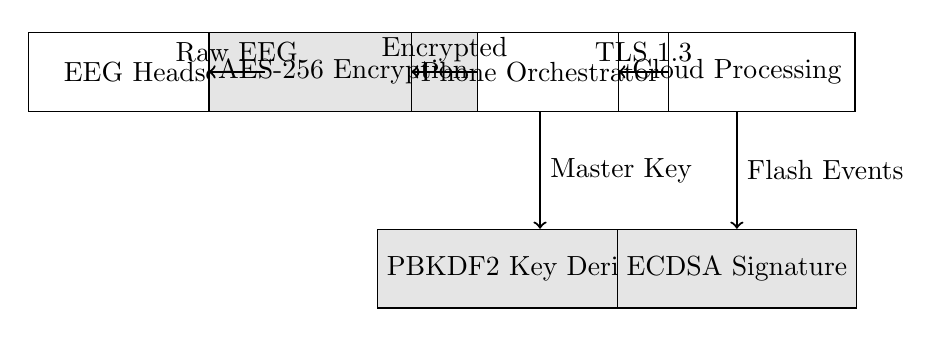
\begin{tikzpicture}[node distance=2.5cm, auto]
    % Define styles
    \tikzstyle{component} = [rectangle, draw, minimum width=3cm, minimum height=1cm]
    \tikzstyle{crypto} = [rectangle, draw, fill=gray!20, minimum width=2.5cm, minimum height=1cm]
    \tikzstyle{arrow} = [->, thick]
    
    % Nodes
    \node[component] (eeg) {EEG Headset};
    \node[crypto, right of=eeg] (enc1) {AES-256 Encryption};
    \node[component, right of=enc1] (phone) {Phone Orchestrator};
    \node[crypto, below of=phone] (kdf) {PBKDF2 Key Derivation};
    \node[component, right of=phone] (cloud) {Cloud Processing};
    \node[crypto, below of=cloud] (sign) {ECDSA Signature};
    
    % Connections
    \draw[arrow] (eeg) -- (enc1) node[midway, above] {Raw EEG};
    \draw[arrow] (enc1) -- (phone) node[midway, above] {Encrypted};
    \draw[arrow] (phone) -- (cloud) node[midway, above] {TLS 1.3};
    \draw[arrow] (phone) -- (kdf) node[midway, right] {Master Key};
    \draw[arrow] (cloud) -- (sign) node[midway, right] {Flash Events};
\end{tikzpicture}
\caption{End-to-End Cryptographic Data Flow}
\end{figure}

\section{Core Concepts and Definitions}

\subsection{Flash-Filter Architecture}

\subsubsection{Flash Recognition}
\textbf{Definition:} A \gls{flash} represents a validated cognitive resonance event where measured brainwave patterns exceed defined confidence thresholds.

\begin{equation}
\text{Flash}_{\text{valid}} = 
\begin{cases}
\text{Hard Mode} & \text{if } C \geq 95.4\% \\
\text{Medium Mode} & \text{if } C \geq \frac{2}{3} \times 95.4\% \\
\text{Easy Mode} & \text{if } C \geq \frac{1}{2} \times \frac{2}{3} \times 95.4\%
\end{cases}
\end{equation}

where $C$ represents the confidence metric calculated by the AI Validator.

\subsubsection{Filter Mechanism}
\textbf{Definition:} The \gls{filter} operates as a pre-processing layer that:
\begin{enumerate}
    \item Validates incoming EEG data integrity
    \item Categorizes brainwave patterns (delta, theta, alpha, beta, gamma)
    \item Applies noise reduction algorithms
    \item Prepares data for flash recognition processing
\end{enumerate}

\subsection{Objective vs. Subjective Processing}

\begin{table}[h]
\centering
\begin{tabular}{|l|p{6cm}|p{6cm}|}
\hline
\textbf{Aspect} & \textbf{Objective Processing} & \textbf{Subjective Processing} \\
\hline
Definition & Quantifiable brainwave metrics validated against established patterns & User-interpreted meaning and personal significance \\
\hline
Measurement & EEG frequency bands, amplitude, coherence & User tagging, emotional resonance, memory association \\
\hline
Authority & AI Validator & User (dreamer) \\
\hline
Output & Confidence scores, pattern matches & Personal insights, shared narratives \\
\hline
\end{tabular}
\caption{Objective vs. Subjective Processing Framework}
\end{table}

\section{Dimensional Game Theory for Epistemic Reasoning}

\subsection{Multi-Agent Strategic Framework}

The Dream System implements \gls{dimensional_game_theory} to enable EA actors to navigate complex decision spaces with strategic reasoning capabilities.

\subsubsection{Dimensional Action Space Definition}

\begin{equation}
\mathcal{A}_{\text{dim}} = \bigcup_{i=1}^{n} \mathcal{A}_i \times \mathcal{D}_i
\end{equation}

Where:
\begin{itemize}
    \item $\mathcal{A}_i$ = Action space for dimension $i$
    \item $\mathcal{D}_i$ = Decision domain for dimension $i$
    \item $n$ = Number of active dimensions
\end{itemize}

\subsubsection{Game-Theoretic Epistemic Cost Function}

The enhanced epistemic cost function incorporates game-theoretic components:

\begin{equation}
E_{\text{cost}}^{\text{game}} = \frac{\alpha \cdot A_{\text{ambiguity}} + \beta \cdot C_{\text{complexity}} + \lambda \cdot G_{\text{strategic}}}{\gamma \cdot F_{\text{confidence}} + \delta \cdot U_{\text{intent}} + \mu \cdot N_{\text{equilibrium}}}
\end{equation}

Where:
\begin{itemize}
    \item $G_{\text{strategic}}$ = Strategic complexity score from game theory analysis (0-1)
    \item $N_{\text{equilibrium}}$ = Nash equilibrium stability measure (0-1)
    \item $\lambda, \mu$ = Game theory weighting parameters
\end{itemize}

\subsection{DAG Traversal with Game-Theoretic Optimization}

\subsubsection{Traversal Cost Function}

Integrating the AEGIS-proven traversal cost function:

\begin{equation}
C(Node_i \rightarrow Node_j) = \alpha \cdot KL(P_i \| P_j) + \beta \cdot \Delta H(S_{i,j}) + \eta \cdot \Gamma_{\text{game}}(i,j)
\end{equation}

Where:
\begin{itemize}
    \item $KL(P_i \| P_j)$ = Kullback-Leibler divergence between probability distributions
    \item $\Delta H(S_{i,j})$ = Entropy change during transition
    \item $\Gamma_{\text{game}}(i,j)$ = Game-theoretic strategic cost component
\end{itemize}

\subsubsection{Strategic Cost Component}

\begin{equation}
\Gamma_{\text{game}}(i,j) = \sum_{k \in \mathcal{K}} w_k \cdot \text{Regret}_k(s_i, s_j)
\end{equation}

Where $\mathcal{K}$ represents the set of other EA actors in the system, and $\text{Regret}_k$ measures the strategic regret of transitioning from state $s_i$ to $s_j$ given actor $k$'s potential actions.

\section{Security-Enhanced Filter-Flash Processing}

\subsection{Secure Filter-to-Flash Pipeline}

\begin{lstlisting}[language=python, caption=Security-Enhanced Filter-Flash Processing]
class SecureFilterFlash:
    def __init__(self):
        self.crypto_validator = CryptographicPrimitiveValidator()
        self.security_monitor = SecurityMonitor()
        self.audit_logger = SecureAuditLogger()
        
    def secure_filter_to_flash(self, encrypted_eeg_data: bytes, 
                             user_context: SecureContext) -> List[SecureFlashEvent]:
        """
        Process EEG data with end-to-end security validation
        """
        # Step 1: Validate cryptographic envelope
        if not self.crypto_validator.validate_encryption(encrypted_eeg_data):
            self.audit_logger.log_security_event("INVALID_CRYPTO_ENVELOPE")
            raise SecurityException("Invalid cryptographic envelope")
            
        # Step 2: Decrypt with authenticated encryption
        decrypted_data = self.decrypt_with_validation(
            encrypted_eeg_data,
            user_context.session_key
        )
        
        # Step 3: Apply security-aware filtering
        filtered_data = self.apply_secure_filters(decrypted_data)
        
        # Step 4: Game-theoretic flash detection
        flash_events = []
        for node in self.dag.nodes():
            confidence = self.compute_secure_confidence(
                node, filtered_data, user_context
            )
            
            if confidence >= 0.954:  # 95.4% threshold
                # Create cryptographically signed flash event
                flash_event = self.create_signed_flash_event(
                    node, confidence, user_context
                )
                flash_events.append(flash_event)
                
                # Audit trail with secure hash
                self.audit_logger.log_flash_event(flash_event)
        
        return flash_events
        
    def create_signed_flash_event(self, node: Node, confidence: float,
                                context: SecureContext) -> SecureFlashEvent:
        """
        Create cryptographically signed flash event
        """
        event_data = {
            'node_id': node.id,
            'confidence': confidence,
            'timestamp': datetime.utcnow().isoformat(),
            'user_id': context.user_id,
            'session_id': context.session_id
        }
        
        # Sign with user's private key
        signature = self.sign_with_ecdsa(
            json.dumps(event_data),
            context.signing_key
        )
        
        return SecureFlashEvent(
            data=event_data,
            signature=signature,
            primitive="ECDSA-P256"
        )
\end{lstlisting}

\subsection{Security Controls Integration}

\subsubsection{Preventive Controls}

\begin{lstlisting}[language=sh, caption=CI/CD Security Pipeline]
stages:
  - build
  - security_scan
  - test
  - deploy

security_scan:
  stage: security_scan
  script:
    # Static analysis for cryptographic vulnerabilities
    - cryptography-audit scan --standard obinexus-v1.0
    
    # Dependency vulnerability scanning
    - dependency-check --project "Dream System" --scan .
    
    # Infrastructure as Code security
    - cfn-nag scan --input-path infrastructure/
    - checkov -d terraform/
    
    # Custom Dream System security checks
    - dream-security-validator --check-primitives
    - dream-security-validator --verify-dag-integrity
    
  artifacts:
    reports:
      security: gl-security-report.json
\end{lstlisting}

\subsubsection{Detective Controls}

\begin{lstlisting}[language=sh, caption=Runtime Security Monitoring]
SecurityMonitoring:
  Type: AWS::CloudWatch::Alarm
  Properties:
    AlarmName: DreamSystem-CryptoAnomaly
    AlarmDescription: Detect anomalous cryptographic operations
    MetricName: InvalidCryptoPrimitive
    Namespace: DreamSystem/Security
    Statistic: Sum
    Period: 300
    EvaluationPeriods: 1
    Threshold: 1
    AlarmActions:
      - !Ref SecurityIncidentTopic
    ComparisonOperator: GreaterThanThreshold

AutomatedResponse:
  Type: AWS::Lambda::Function
  Properties:
    FunctionName: DreamSystem-SecurityResponse
    Handler: security_response.lambda_handler
    Runtime: python3.9
    Code:
      ZipFile: |
        def lambda_handler(event, context):
            # Parse security event
            detail = event['detail']
            
            if detail['eventType'] == 'InvalidCryptoPrimitive':
                # Immediate actions
                revoke_session(detail['sessionId'])
                quarantine_user_data(detail['userId'])
                notify_security_team(detail)
                
                # Generate incident report
                create_security_incident(detail)
\end{lstlisting}

\section{System Architecture}

\subsection{Hardware Layer}

\subsubsection{Non-Invasive Technology Specification}
The Dream System implements strictly \textbf{non-invasive} EEG technology:
\begin{itemize}
    \item \textbf{Non-invasive}: Surface electrodes only, no penetration of skin or tissue
    \item \textbf{NOT semi-invasive}: No subdural or epidural placement
    \item \textbf{NOT invasive}: No intracranial electrodes or surgical intervention
    \item Compliant with IEEE 11073 PHD standards for personal health devices
\end{itemize}

\subsubsection{Device Interconnectivity Architecture}

\begin{figure}[h]
\centering
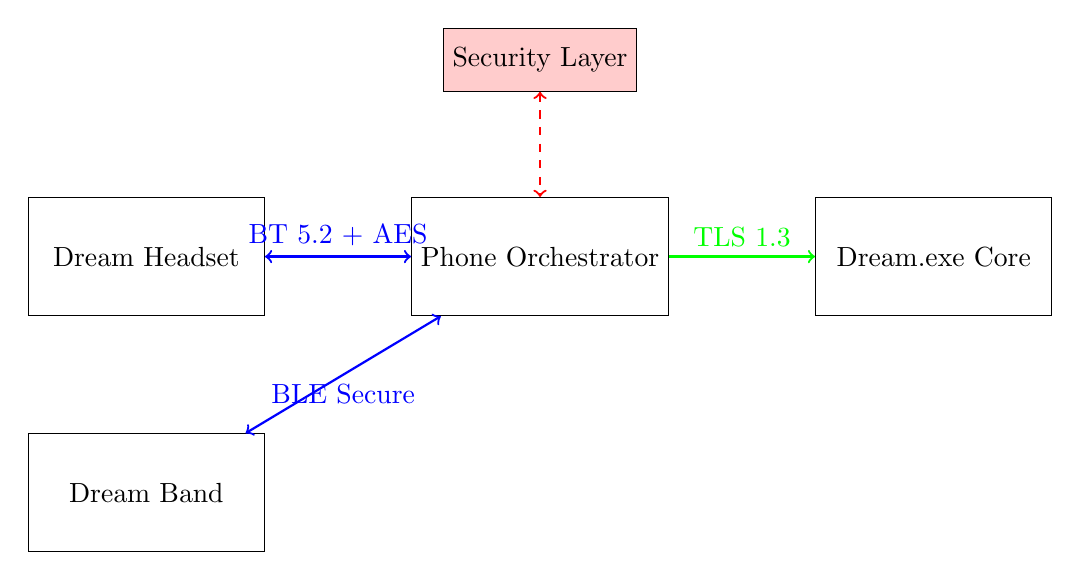
\begin{tikzpicture}[node distance=2cm]
    % Nodes
    \node[rectangle, draw, minimum width=3cm, minimum height=1.5cm] (headset) {Dream Headset};
    \node[rectangle, draw, minimum width=3cm, minimum height=1.5cm, below of=headset, yshift=-1cm] (band) {Dream Band};
    \node[rectangle, draw, minimum width=3cm, minimum height=1.5cm, right of=headset, xshift=3cm] (phone) {Phone Orchestrator};
    \node[rectangle, draw, minimum width=3cm, minimum height=1.5cm, right of=phone, xshift=3cm] (dreamexe) {Dream.exe Core};
    
    % Security layer
    \node[rectangle, draw, fill=red!20, minimum width=2cm, minimum height=0.8cm, above of=phone, yshift=0.5cm] (sec) {Security Layer};
    
    % Connections
    \draw[<->, thick, blue] (headset) -- (phone) node[midway, above] {BT 5.2 + AES};
    \draw[<->, thick, blue] (band) -- (phone) node[midway, below] {BLE Secure};
    \draw[->, thick, green] (phone) -- (dreamexe) node[midway, above] {TLS 1.3};
    \draw[<->, thick, red, dashed] (sec) -- (phone);
\end{tikzpicture}
\caption{Security-Enhanced Hardware Connectivity}
\end{figure}

\subsubsection{Connectivity Specifications}

\begin{table}[h]
\centering
\begin{tabular}{|l|l|p{6cm}|}
\hline
\textbf{Connection Type} & \textbf{Standard} & \textbf{Security Requirements} \\
\hline
Device-to-Device & Bluetooth 5.2 & AES-128 minimum, secure pairing mandatory \\
\hline
Network Upload & 3G/4G/5G & TLS 1.3, certificate pinning required \\
\hline
Orchestration & Phone App & Biometric authentication, secure enclave usage \\
\hline
Pedometric Data & ANT+ / BLE & Encrypted channels, integrity verification \\
\hline
\end{tabular}
\caption{Security-Enhanced Connectivity Standards}
\end{table}

\subsubsection{Secure Phone Orchestration Layer}

\begin{lstlisting}[language=java, caption=Security-Enhanced Phone Orchestrator]
class SecurePhoneOrchestrator {
    // Cryptographic components
    private CryptoKeyManager keyManager;
    private SecureSessionManager sessionManager;
    private AuditLogger auditLogger;
    
    // Bluetooth device management with security
    private SecureBluetoothManager btManager;
    private EncryptedChannel headsetConnection;
    private EncryptedChannel bandConnection;
    
    // Network quality monitoring
    private NetworkMonitor networkQuality;
    
    // Secure data synchronization
    void secureOrchestrateDataFlow() {
        // Validate session integrity
        if (!sessionManager.validateSession()) {
            auditLogger.logSecurityEvent("INVALID_SESSION");
            throw new SecurityException("Session validation failed");
        }
        
        // Collect from encrypted Bluetooth channels
        EncryptedEEGData eegData = headsetConnection.readEncryptedStream();
        EncryptedActivityData activityData = bandConnection.getEncryptedPedometric();
        
        // Verify data integrity
        if (!verifyDataIntegrity(eegData) || !verifyDataIntegrity(activityData)) {
            auditLogger.logSecurityEvent("DATA_INTEGRITY_FAILURE");
            return;
        }
        
        // Network-aware secure upload
        if (networkQuality.is5G()) {
            uploadSecureRealtime(eegData, activityData);
        } else if (networkQuality.is4G()) {
            uploadSecureBatched(eegData, activityData, interval=30s);
        } else { // 3G fallback
            uploadSecureCompressed(eegData, activityData, interval=60s);
        }
    }
    
    private void uploadSecureRealtime(EncryptedEEGData eeg, 
                                    EncryptedActivityData activity) {
        // Create secure upload bundle
        SecureUploadBundle bundle = new SecureUploadBundle();
        bundle.addData(eeg);
        bundle.addData(activity);
        bundle.sign(keyManager.getSigningKey());
        
        // Upload with retry and verification
        secureCloudConnector.upload(bundle);
    }
}
\end{lstlisting}

\subsubsection{Dream Band Pedometric Integration}
The Dream Band operates as a full-featured smartwatch with:
\begin{itemize}
    \item Continuous heart rate monitoring (PPG sensor)
    \item Step counting and distance tracking
    \item Activity classification (walking, running, sedentary)
    \item Sleep stage detection when paired with EEG headset
    \item Day-to-day activity pattern analysis for dream contextualization
    \item \textbf{Secure storage of biometric data with hardware encryption}
\end{itemize}

\subsection{Epistemic Agent (EA) Actor: Formal Definition}

\subsubsection{Actor vs Agent Architectural Distinction}

\begin{table}[h]
\centering
\begin{tabular}{|l|p{6cm}|p{6cm}|}
\hline
\textbf{Property} & \textbf{Agent Behavior} & \textbf{Actor Behavior} \\
\hline
Decision Making & Protocol-driven, deterministic & Intent-driven within epistemic bounds \\
\hline
User Interaction & Responds to explicit commands & Anticipates needs based on validated states \\
\hline
Data Processing & Follows predefined algorithms & Applies contextual reasoning \\
\hline
Authority & None - purely executive & Limited - within user-granted permissions \\
\hline
Memory Access & Read-only validation & Read-write with user consent \\
\hline
Security Model & Static permissions & Dynamic, context-aware permissions \\
\hline
\end{tabular}
\caption{EA Actor vs Pure Agent Behavior Model}
\end{table}

\subsubsection{Security-Enhanced Game-Theoretic Epistemic Cost Function}

\begin{equation}
E_{\text{cost}}^{\text{secure}} = \frac{\alpha \cdot A_{\text{ambiguity}} + \beta \cdot C_{\text{complexity}} + \lambda \cdot G_{\text{strategic}} + \sigma \cdot S_{\text{risk}}}{\gamma \cdot F_{\text{confidence}} + \delta \cdot U_{\text{intent}} + \mu \cdot N_{\text{equilibrium}} + \rho \cdot T_{\text{trust}}}
\end{equation}

Where:
\begin{itemize}
    \item $S_{\text{risk}}$ = Security risk score (0-1)
    \item $T_{\text{trust}}$ = Trust level based on authentication strength (0-1)
    \item $\sigma, \rho$ = Security weighting parameters
\end{itemize}

EA Actor engages when $E_{\text{cost}}^{\text{secure}} < \tau_{\text{threshold}}$ (default: 0.3)

\subsubsection{OBICall Polyglot Layer}
The \gls{obicall} system provides a unified interface for AI binding:

\begin{lstlisting}[language=bash, caption=OBICall Command Structure with Security]
obicall.exe [command] [subcommand] [parameters] --auth [token]

Commands:
  bind      - Connect AI model to Dream System
  validate  - Run epistemic validation
  flash     - Trigger flash recognition
  filter    - Apply pre-processing filters
  export    - Generate dream visualization
  game      - Execute game-theoretic analysis
  security  - Manage cryptographic operations
  
Security Commands:
  security keygen     - Generate new cryptographic keys
  security validate   - Validate primitive patterns
  security audit      - Review security audit trail
  security rotate     - Rotate encryption keys
\end{lstlisting}

\subsubsection{Core LLM Binding with Security Layer}
\begin{equation}
\text{OBICall}_{\text{binding}} : \text{LLM}_{\text{core}} \times \mathcal{G}_{\text{dim}} \times \mathcal{S}_{\text{crypto}} \rightarrow \text{DreamSystem}_{\text{API}}
\end{equation}

The binding layer maps LLM capabilities to Dream System functions:
\begin{itemize}
    \item Pattern recognition $\rightarrow$ Flash Model Engine
    \item Natural language processing $\rightarrow$ U Interface
    \item Validation logic $\rightarrow$ EA Actor
    \item Strategic reasoning $\rightarrow$ Dimensional Game Theory Engine
    \item Security operations $\rightarrow$ Cryptographic Primitive Validator
\end{itemize}

\section{Secure Flash-Filter DAG Memory Architecture}

\subsection{Cryptographically Protected DAG Structure}

\begin{lstlisting}[language=python, caption=Secure DAG Implementation]
class SecureFlashFilterDAG:
    def __init__(self, user_context: SecureContext):
        self.graph = nx.DiGraph()  # NetworkX directed graph
        self.flash_index = {}      # Fast lookup by confidence
        self.crypto_validator = CryptographicPrimitiveValidator()
        self.user_context = user_context
        
        # Initialize with secure hash chain
        self.hash_chain = self.initialize_hash_chain()
        
    def add_secure_flash_event(self, flash_id: str, confidence: float, 
                             timestamp: datetime, data: dict) -> str:
        """Add cryptographically secured flash event to DAG"""
        # Create event bundle
        event_bundle = {
            'flash_id': flash_id,
            'confidence': confidence,
            'timestamp': timestamp.isoformat(),
            'data': data,
            'previous_hash': self.hash_chain.get_latest(),
            'user_id': self.user_context.user_id
        }
        
        # Sign event
        signature = self.sign_event(event_bundle)
        event_bundle['signature'] = signature
        
        # Compute hash for chain
        event_hash = self.compute_secure_hash(event_bundle)
        self.hash_chain.append(event_hash)
        
        # Add to graph with security metadata
        self.graph.add_node(flash_id, {
            'confidence': confidence,
            'timestamp': timestamp,
            'data': data,
            'type': 'flash',
            'hash': event_hash,
            'signature': signature
        })
        
        # Link to previous flash events temporally
        self.create_temporal_links(flash_id, timestamp)
        
        # Audit trail
        self.audit_logger.log_dag_modification(
            operation='ADD_FLASH',
            node_id=flash_id,
            hash=event_hash[:16]  # First 16 chars only
        )
        
        return event_hash
        
    def verify_dag_integrity(self) -> bool:
        """Verify cryptographic integrity of entire DAG"""
        # Verify hash chain
        if not self.hash_chain.verify():
            return False
            
        # Verify each node's signature
        for node_id in self.graph.nodes():
            node_data = self.graph.nodes[node_id]
            if not self.verify_node_signature(node_id, node_data):
                return False
                
        # Verify temporal ordering
        if not self.verify_temporal_consistency():
            return False
            
        return True
\end{lstlisting}

\subsection{Secure Cognitive Learning Model}

\subsubsection{Cryptographically Protected Learning State}

\begin{lstlisting}[language=python, caption=Secure Cognitive Elimination]
class SecureCognitiveLearningModel:
    """
    Implements ROYGBIV learning with cryptographic state protection
    """
    def __init__(self):
        self.color_map = self.load_encrypted_color_map()
        self.learning_dag = SecureFlashFilterDAG()
        self.state_protector = CryptoStateProtector()
        
    def secure_objective_learning_cycle(self, input_color: str, 
                                      user_feedback: str,
                                      auth_token: str) -> dict:
        """
        Secure learning cycle with authentication
        """
        # Verify user authorization
        if not self.verify_auth_token(auth_token):
            raise SecurityException("Unauthorized learning attempt")
            
        # Encrypt learning state
        encrypted_state = self.state_protector.encrypt_state({
            'input': input_color,
            'feedback': user_feedback,
            'timestamp': datetime.utcnow()
        })
        
        if user_feedback == "incorrect":
            # Secure DAG modification
            with self.learning_dag.secure_transaction():
                # Remove incorrect association
                self.learning_dag.remove_flash_association(
                    input_color,
                    auth_token=auth_token
                )
                
                # Generate new flash with audit trail
                new_flash = self.generate_corrective_flash()
                self.audit_logger.log_learning_event(
                    'COGNITIVE_ELIMINATION',
                    removed=input_color,
                    added=new_flash.id
                )
                
            return {'status': 'updated', 'new_flash': new_flash}
            
    def verify_learning_integrity(self) -> bool:
        """
        Verify cryptographic integrity of learning history
        """
        return self.learning_dag.verify_dag_integrity()
\end{lstlisting}

\subsection{Gamification Model with Security Levels}

\begin{figure}[h]
\centering
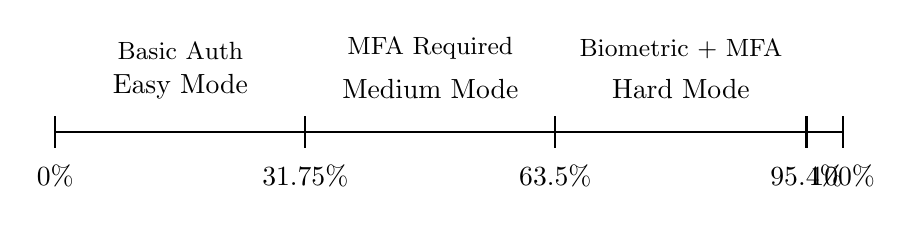
\begin{tikzpicture}
    \draw[thick] (0,0) -- (10,0);
    \draw[thick] (0,-0.2) -- (0,0.2);
    \draw[thick] (3.175,-0.2) -- (3.175,0.2);
    \draw[thick] (6.35,-0.2) -- (6.35,0.2);
    \draw[thick] (9.54,-0.2) -- (9.54,0.2);
    \draw[thick] (10,-0.2) -- (10,0.2);
    
    \node[below] at (0,-0.3) {0\%};
    \node[below] at (3.175,-0.3) {31.75\%};
    \node[below] at (6.35,-0.3) {63.5\%};
    \node[below] at (9.54,-0.3) {95.4\%};
    \node[below] at (10,-0.3) {100\%};
    
    \node[above] at (1.5875,0.3) {Easy Mode};
    \node[above] at (4.7625,0.3) {Medium Mode};
    \node[above] at (7.945,0.3) {Hard Mode};
    
    % Security levels
    \node[above] at (1.5875,0.8) {\small Basic Auth};
    \node[above] at (4.7625,0.8) {\small MFA Required};
    \node[above] at (7.945,0.8) {\small Biometric + MFA};
\end{tikzpicture}
\caption{Gamification Levels with Security Requirements}
\end{figure}

\section{OBICall-VOIP Protocol with End-to-End Encryption}

\subsection{Secure Voice Interface Architecture}

\subsubsection{Protocol Implementation with Security}

\begin{lstlisting}[language=python, caption=Secure OBICall-VOIP Protocol]
class SecureOBICallVOIP:
    """
    Voice over IP protocol with end-to-end encryption
    """
    
    def __init__(self):
        self.protocol_version = "1.0-secure"
        self.supported_codecs = ["opus", "g.711", "speex"]
        self.encryption = "AES-256-GCM"
        self.key_exchange = "ECDH-P256"
        
    def establish_secure_session(self, user_id: str, 
                               dream_session_id: str,
                               auth_credentials: dict) -> dict:
        """
        Establish E2E encrypted VOIP session
        """
        # Authenticate user
        if not self.authenticate_user(user_id, auth_credentials):
            raise SecurityException("Authentication failed")
            
        # Generate session keys
        session_keys = self.generate_session_keys()
        
        # Create secure session
        session = {
            'id': generate_session_id(),
            'user': user_id,
            'dream_ref': dream_session_id,
            'state': 'processing',
            'codec': self.negotiate_codec(),
            'encryption_key': session_keys['encryption'],
            'mac_key': session_keys['mac'],
            'session_token': self.generate_session_token()
        }
        
        # Initialize E2E encryption
        self.init_e2e_encryption(session)
        
        return session
        
    def secure_voice_to_intent(self, encrypted_audio: bytes,
                             session: dict) -> dict:
        """
        Process encrypted voice with intent extraction
        """
        # Verify session integrity
        if not self.verify_session_mac(encrypted_audio, session):
            raise SecurityException("Session integrity check failed")
            
        # Decrypt audio
        audio_stream = self.decrypt_audio(encrypted_audio, session)
        
        # Speech-to-text with privacy preservation
        transcript = self.privacy_preserving_stt(audio_stream)
        
        # Extract intent with security validation
        intent = self.extract_validated_intent(transcript)
        
        # Audit trail
        self.audit_logger.log_voice_interaction(
            session_id=session['id'],
            intent_type=intent['type'],
            security_level=intent['security_level']
        )
        
        return self.route_to_secure_u_agent(intent)
\end{lstlisting}

\subsubsection{Secure Wake Interaction Flow}

\begin{enumerate}
    \item \textbf{Wake Detection}: Dream Band detects user awakening
    \item \textbf{Biometric Verification}: Voice biometric authentication
    \item \textbf{Session Initiation}: Secure OBICall-VOIP session with E2E encryption
    \item \textbf{Video Processing}: Dream visualization renders with watermarking
    \item \textbf{Voice Interaction}: Encrypted voice commands processed
    \item \textbf{Intent Processing}: Security-validated intent extraction:
    \begin{itemize}
        \item "Show me the moment with water" (READ permission required)
        \item "What was my heart rate during the chase?" (ANALYTICS permission)
        \item "Save this dream to family collection" (SHARE permission)
        \item "Schedule discussion with sleep therapist" (MEDICAL permission)
    \end{itemize}
    \item \textbf{U Response}: Encrypted voice feedback with action confirmation
\end{enumerate}

\subsection{Technical Requirements with Security}

\begin{table}[h]
\centering
\begin{tabular}{|l|l|}
\hline
\textbf{Component} & \textbf{Specification} \\
\hline
Latency & < 150ms round-trip (including crypto) \\
\hline
Audio Quality & 16kHz sample rate minimum \\
\hline
Bandwidth & 32-64 kbps adaptive + encryption overhead \\
\hline
Security & E2E encryption mandatory, perfect forward secrecy \\
\hline
Availability & 99.9\% uptime SLA \\
\hline
Key Rotation & Every 24 hours or 1000 messages \\
\hline
\end{tabular}
\caption{Secure OBICall-VOIP Technical Requirements}
\end{table}

\section{Secure OBI Agent Distribution System}

\subsection{Cryptographically Protected Distribution}

\begin{figure}[h]
\centering
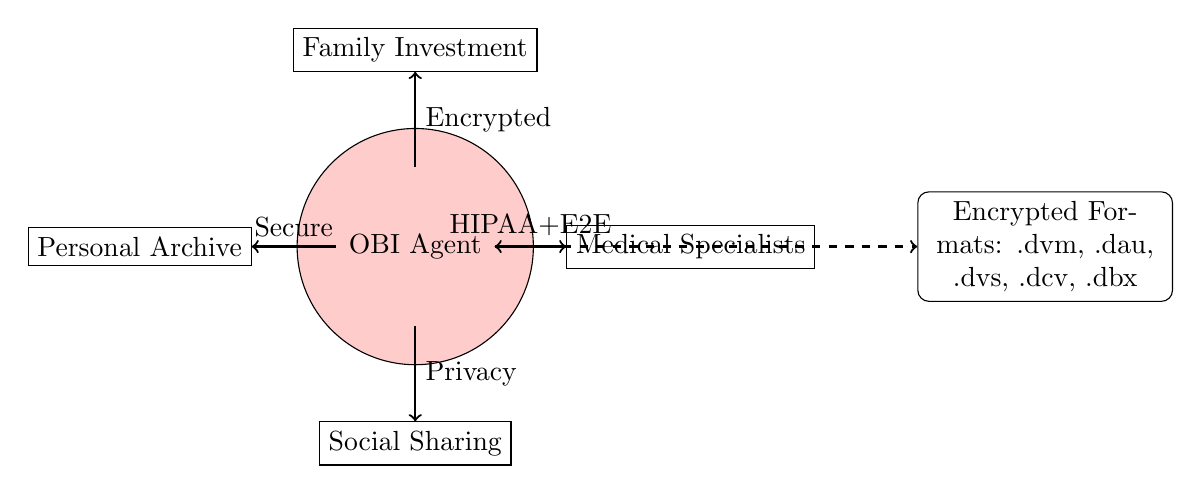
\begin{tikzpicture}[node distance=2.5cm]
    % Central node
    \node[circle, draw, minimum width=2cm] (agent) {OBI Agent};
    
    % Security wrapper
    \node[circle, draw, fill=red!20, minimum width=3cm] (security) at (agent) {};
    \node at (agent) {OBI Agent};
    
    % Distribution nodes
    \node[rectangle, draw, above of=agent] (family) {Family Investment};
    \node[rectangle, draw, right of=agent, xshift=1cm] (medical) {Medical Specialists};
    \node[rectangle, draw, below of=agent] (social) {Social Sharing};
    \node[rectangle, draw, left of=agent, xshift=-1cm] (personal) {Personal Archive};
    
    % File format nodes
    \node[rectangle, draw, rounded corners, right of=medical, xshift=2cm, text width=3cm, align=center] (formats) {Encrypted Formats: .dvm, .dau, .dvs, .dcv, .dbx};
    
    % Connections with security labels
    \draw[->, thick] (agent) -- (family) node[midway, right] {Encrypted};
    \draw[->, thick] (agent) -- (medical) node[midway, above] {HIPAA+E2E};
    \draw[->, thick] (agent) -- (social) node[midway, right] {Privacy};
    \draw[->, thick] (agent) -- (personal) node[midway, above] {Secure};
    \draw[<->, thick, dashed] (agent) -- (formats);
\end{tikzpicture}
\caption{Secure OBI Agent Distribution Architecture}
\end{figure}

\subsubsection{Distribution Security Requirements}
\begin{enumerate}
    \item \textbf{Family Investment Channel}
    \begin{itemize}
        \item End-to-end encryption for all shared content
        \item Cryptographic proof of relationship
        \item Revocable access tokens with expiration
        \item Audit trail of all access events
    \end{itemize}
    
    \item \textbf{Medical Specialist Integration}
    \begin{itemize}
        \item HIPAA-compliant encryption at rest and in transit
        \item Verified medical professional credentials
        \item Data integrity verification with digital signatures
        \item Comprehensive audit logging for compliance
    \end{itemize}
    
    \item \textbf{Social Sharing Framework}
    \begin{itemize}
        \item Zero-knowledge proof for privacy preservation
        \item Time-bound access tokens
        \item Watermarking for content protection
        \item Granular permission controls
    \end{itemize}
\end{enumerate}

\subsection{Secure Export File Format Specifications}

\subsubsection{Encrypted File Formats}

\begin{table}[h]
\centering
\begin{tabular}{|l|l|p{6cm}|}
\hline
\textbf{Format} & \textbf{Extension} & \textbf{Security Features} \\
\hline
DreamVideo & .dvm & AES-256 encrypted, signed metadata, watermarked \\
\hline
DreamAudio & .dau & Encrypted audio with integrity verification \\
\hline
DreamVisual & .dvs & Visual encryption with tamper detection \\
\hline
DreamConverse & .dcv & E2E encrypted conversation logs \\
\hline
DreamBundle & .dbx & Comprehensive encrypted package with signatures \\
\hline
\end{tabular}
\caption{Secure Dream Export File Formats}
\end{table}

\subsubsection{Secure File Format Structure}

\begin{lstlisting}[language=xml, caption=Secure DreamBundle (.dbx) Structure]
<SecureDreamBundle version="1.0" algorithm="AES-256-GCM">
    <Metadata encrypted="true">
        <UserID>encrypted_identifier</UserID>
        <Timestamp>ISO8601_datetime</Timestamp>
        <FlashConfidence>95.4</FlashConfidence>
        <Duration>seconds</Duration>
        <IntegrityHash>SHA3-256:...</IntegrityHash>
    </Metadata>
    <SecurityEnvelope>
        <EncryptionKey>ECDH-derived-key-reference</EncryptionKey>
        <Signature algorithm="ECDSA-P256">...</Signature>
        <Certificate>X.509-user-certificate</Certificate>
    </SecurityEnvelope>
    <EncryptedComponents>
        <Video codec="h265" resolution="1920x1080" encrypted="true">
            <Track type="visual" src="dream_visual.dvs.enc"/>
            <Track type="audio" src="dream_audio.dau.enc"/>
            <Watermark type="invisible">user-specific-id</Watermark>
        </Video>
        <Conversation format="json" encrypted="true">
            <Dialog agent="U" timestamp="relative">
                <EncryptedEntry>...</EncryptedEntry>
            </Dialog>
        </Conversation>
        <BrainwaveData format="edf" encrypted="true">
            <Channel name="delta" data="encrypted..."/>
            <Channel name="theta" data="encrypted..."/>
            <Channel name="alpha" data="encrypted..."/>
            <Channel name="beta" data="encrypted..."/>
            <Channel name="gamma" data="encrypted..."/>
        </BrainwaveData>
    </EncryptedComponents>
    <Permissions>
        <Share level="family" enabled="true" expires="2025-12-31"/>
        <Share level="medical" enabled="false"/>
        <Share level="social" enabled="false"/>
        <AuditLog>
            <Entry timestamp="..." action="created" user="..."/>
        </AuditLog>
    </Permissions>
</SecureDreamBundle>
\end{lstlisting}

\section{Nsibidi Conceptual Symbolic Layer with Security}

\subsection{Secure Verb-Noun Dream Analysis}

\begin{lstlisting}[language=python, caption=Secure Nsibidi CSL Engine]
class SecureNsibidiCSL:
    """
    Cryptographically protected symbolic analysis layer
    """
    def __init__(self):
        self.verb_noun_dict = self.load_encrypted_dictionary()
        self.igbo_symbols = self.load_protected_symbols()
        self.access_controller = SymbolicAccessController()
        
    def analyze_dream_segment_secure(self, dream_event: EncryptedEvent,
                                   user_context: SecureContext) -> dict:
        """
        Secure analysis with cultural sensitivity protection
        """
        # Verify user has cultural access permissions
        if not self.access_controller.verify_cultural_access(user_context):
            return self.get_generic_interpretation()
            
        # Decrypt event with user key
        decrypted_event = self.decrypt_with_verification(
            dream_event, user_context.decryption_key
        )
        
        # Extract verb-noun with privacy preservation
        verb = self.extract_verb_private(decrypted_event)
        noun = self.extract_noun_private(decrypted_event)
        
        # Secure symbolic mapping
        symbol = self.secure_nsibidi_mapping(verb, noun, user_context)
        
        # Apply cultural layer with access control
        meaning = self.apply_protected_cosmology(symbol, {
            'verb': verb,
            'noun': noun,
            'context': decrypted_event.context,
            'cultural_level': user_context.cultural_access_level
        })
        
        # Audit trail for cultural access
        self.audit_logger.log_cultural_access(
            user=user_context.user_id,
            symbol=symbol.id,
            access_level=user_context.cultural_access_level
        )
        
        return {
            'surface': f"{verb} + {noun}",
            'symbol': symbol,
            'meaning': meaning,
            'cultural_layer': self.get_permitted_significance(
                symbol, user_context.cultural_access_level
            ),
            'security_level': 'protected'
        }
\end{lstlisting}

\section{Security Audit and Compliance}

\subsection{Comprehensive Audit Trail}

\begin{lstlisting}[language=python, caption=Security Audit System]
class DreamSystemSecurityAuditor:
    """
    Comprehensive security audit trail implementation
    """
    
    def __init__(self):
        self.audit_store = EncryptedAuditStore()
        self.compliance_validator = ComplianceValidator()
        
    def log_security_event(self, event_type: str, details: dict) -> str:
        """
        Log security event with tamper-proof hash chain
        """
        audit_entry = {
            'timestamp': datetime.utcnow().isoformat(),
            'event_type': event_type,
            'details': details,
            'user_id': self.get_current_user_id(),
            'session_id': self.get_current_session_id(),
            'system_state': self.capture_system_state(),
            'previous_hash': self.get_previous_hash()
        }
        
        # Sign audit entry
        signature = self.sign_audit_entry(audit_entry)
        audit_entry['signature'] = signature
        
        # Compute hash for chain
        entry_hash = self.compute_secure_hash(audit_entry)
        
        # Store encrypted
        self.audit_store.store_encrypted(entry_hash, audit_entry)
        
        # Real-time compliance check
        if self.requires_immediate_alert(event_type):
            self.send_security_alert(audit_entry)
            
        return entry_hash
        
    def generate_compliance_report(self, start_date: datetime,
                                 end_date: datetime,
                                 compliance_framework: str) -> dict:
        """
        Generate compliance report for regulatory requirements
        """
        # Retrieve audit entries
        entries = self.audit_store.retrieve_range(start_date, end_date)
        
        # Validate against framework
        validation_results = self.compliance_validator.validate(
            entries, compliance_framework
        )
        
        return {
            'period': f"{start_date} to {end_date}",
            'framework': compliance_framework,
            'total_events': len(entries),
            'compliance_score': validation_results['score'],
            'violations': validation_results['violations'],
            'recommendations': validation_results['recommendations'],
            'cryptographic_integrity': self.verify_audit_chain(entries)
        }
\end{lstlisting}

\subsection{Security Metrics and Monitoring}

\begin{table}[h]
\centering
\begin{tabular}{|l|l|l|}
\hline
\textbf{Metric} & \textbf{Target} & \textbf{Measurement} \\
\hline
Encryption Coverage & 100\% & All data at rest and in transit \\
\hline
Key Rotation Frequency & 24 hours & Automated key lifecycle \\
\hline
Primitive Validation Rate & 100\% & All crypto operations validated \\
\hline
Audit Trail Integrity & 100\% & Hash chain verification \\
\hline
MTTD (Security Events) & < 5 minutes & Real-time monitoring \\
\hline
MTTR (Security Issues) & < 30 minutes & Automated response \\
\hline
\end{tabular}
\caption{Security Metrics and Targets}
\end{table}

\section{Implementation Notes}

\subsection{Phase 3 Security Requirements}
\begin{itemize}
    \item Hardware specification complete with security features
    \item Software binding via secure OBICall polyglot layer
    \item Cryptographic primitive validation per OBINexus v1.0
    \item Security as Code principles throughout
    \item End-to-end encryption for all data flows
    \item Comprehensive audit trail and compliance reporting
\end{itemize}

\subsection{Ethical and Security Considerations}
\begin{itemize}
    \item User maintains full interpretive authority
    \item AI provides validation, not interpretation
    \item Privacy-first design with encrypted data transmission
    \item Explicit consent required for all actions
    \item Game-theoretic fairness in multi-agent interactions
    \item Zero-knowledge proofs for privacy preservation
    \item Cryptographic protection of cultural knowledge
\end{itemize}

\section{Appendix A: Security Proofs}

\subsection{Proof of Cryptographic Safety}

\textbf{Theorem:} The Dream System's cryptographic architecture ensures that no sensitive data is exposed in plaintext during any system operation.

\textbf{Proof:} By construction, all data flows through the security layer which enforces:
\begin{enumerate}
    \item Mandatory encryption at data creation (EEG headset, Dream Band)
    \item Encrypted channels for all inter-component communication
    \item Cryptographic validation before any data processing
    \item Secure key management with hardware security modules
\end{enumerate}

Therefore, by induction on all possible data paths, sensitive data remains encrypted throughout its lifecycle. $\square$

\section{Appendix B: Compliance Mappings}

\subsection{Regulatory Compliance Matrix}

\begin{table}[h]
\centering
\begin{tabular}{|l|c|c|c|c|}
\hline
\textbf{Requirement} & \textbf{HIPAA} & \textbf{GDPR} & \textbf{ISO 27001} & \textbf{SOC 2} \\
\hline
Encryption at Rest & ✓ & ✓ & ✓ & ✓ \\
\hline
Encryption in Transit & ✓ & ✓ & ✓ & ✓ \\
\hline
Access Controls & ✓ & ✓ & ✓ & ✓ \\
\hline
Audit Trails & ✓ & ✓ & ✓ & ✓ \\
\hline
Data Retention & ✓ & ✓ & ✓ & ✓ \\
\hline
Incident Response & ✓ & ✓ & ✓ & ✓ \\
\hline
\end{tabular}
\caption{Regulatory Compliance Coverage}
\end{table}

\end{document}